% Created 2024-04-28 Sun 09:32
% Intended LaTeX compiler: pdflatex
\documentclass[11pt,oneside]{memoir}
\makeatletter

\usepackage{answerkey-env}

\ifanswerkey
  \usepackage[forcolorpaper, answerkey]{eqexam}
  \usepackage{vinaya-class-questions}
\else
  \usepackage[forcolorpaper, nosolutions]{eqexam}
  \usepackage[nosolutions]{vinaya-class-questions}
\fi

\proofingsymbolColor{linkred}
\fillinColor{linkred}

\def\maketitle{}

\maxtocdepth{subsection}

\newenvironment{twocols}{%
  \raggedright%
  \setlength{\parindent}{0pt}%
  \setlength{\parskip}{8pt}%
  \fontsize{11}{17}\selectfont%
  \begin{multicols}{2}%
}{%
  \end{multicols}%
}

\newenvironment{widecols}{%
  \hspace*{-0.05\linewidth}\begin{minipage}{1.1\linewidth}%
  \raggedright%
  \setlength{\parindent}{0pt}%
  \setlength{\parskip}{8pt}%
  \fontsize{11}{17}\selectfont%
  \begin{multicols}{2}%
}{%
  \end{multicols}%
  \end{minipage}%
}

\newlength\@tmp@width
\newlength\@tmp@height

\renewcommand*{\printchaptertitleHook}{%
  \AddToShipoutPictureBG*{%
    \put(\LenToUnit{\paperwidth-25mm-\spinemargin},\LenToUnit{\paperheight-95mm}){%
      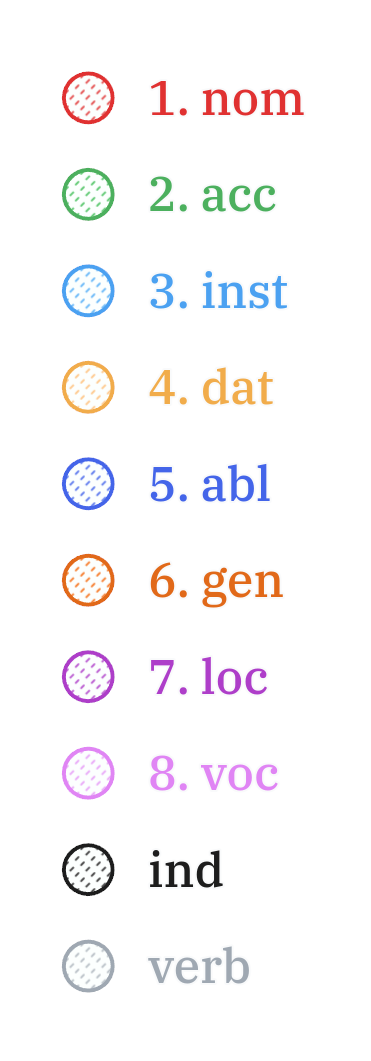
\includegraphics[width=25mm]{./images/cases-legend-white-large.png}%
    }%
  }%
}

\newcommand*\sentenceDiaMsg{\textbf{Exercise:} Draw a sentence analysis diagram below and indicate declensions.}

\newcommand*\sentenceDiaSolution[2][0.4]{%
  \ifanswerkey%
    \hspace*{-\spinemargin}%
    \begin{minipage}{\paperwidth}%
      \centering%
      \includegraphics[scale=#1]{#2}%
    \end{minipage}%
  \else%
    \settototalheight{\@tmp@height}{\includegraphics[scale=#1]{#2}}%
    \begin{minipage}[\@tmp@height]{\linewidth}%
      \sentenceDiaMsg%
    \end{minipage}%
  \fi%
}

\usepackage{cwpuzzle}

\renewcommand\PuzzleCluePre{%
  \begin{minipage}[t]{0.75\linewidth}%
}

\renewcommand\PuzzleClueFont{\fontsize{11}{17}\selectfont}

% \def\PuzzleThickline{\linethickness{2pt}}

\makeatother

\maxtocdepth{section}
\date{\today}
\title{Pali Readings with Sentence Analysis}
\hypersetup{
 pdfauthor={The Bhikkhu Saṅgha},
 pdftitle={Pali Readings with Sentence Analysis},
 pdfkeywords={},
 pdfsubject={},
 pdfcreator={Emacs 29.3 (Org mode 9.6.15)}, 
 pdflang={En_Gb}}
\begin{document}

\maketitle
\frontmatter

{\centering

{\Huge Pāḷi Readings with Sentence Analysis}

\bigskip
\href{https://vinaya-class.github.io}{https://vinaya-class.github.io}

{\scshape\small last updated on}\\
\today

}

\bigskip
\tableofcontents*

\mainmatter

\yournamefalse

\newlength{\colOne}\setlength{\colOne}{0.35\linewidth}
\newlength{\colTwo}\setlength{\colTwo}{0.6\linewidth}

\renewenvironment{quote}%
{\list{}{%
    \doubleLineSize
    \listparindent 0pt
    \itemindent    0pt
    \leftmargin    3em
    \rightmargin   3em
    \parsep        0pt
    \topsep        8pt
    \partopsep     0pt}%
\item[] \raggedright}%
{\endlist}

\chapter{The Weaver's Daughter (Dhp 174 and Comm.)}
\label{sec:org923c637}
\section{Dhp 174 Verse}
\label{sec:org5eea5ce}

\textbf{\textbf{Pesakāradhītāvatthu}}

\begin{itemize}
\item Dhp 174 Verse (\href{https://suttacentral.net/dhp167-178/pli/ms}{SC}, \href{https://www.digitalpalireader.online/\_dprhtml/index.html?loc=k.1.0.0.12.0.0.m}{DPR}, \href{http://localhost:4848/suttas/dhp167-178/pli/ms?quote=Andhabh\%25C5\%25ABto\%2520aya\%25E1\%25B9\%2581\%2520loko\&window\_type=Sutta+Study}{Simsapa})
\item Commentary (\href{https://www.digitalpalireader.online/\_dprhtml/index.html?loc=k.1.0.1.4.6.x.a}{DPR}, \href{http://localhost:4848/suttas/s0502a.att/pli/cst4?quote=andhabh\%25C5\%25ABtoti\%2520ima\%25E1\%25B9\%2581\%2520dhammadesana\%25E1\%25B9\%2581\&window\_type=Sutta+Study}{Simsapa})
\end{itemize}

\begin{quote}
Andhabhūto ayaṁ loko,\\[0pt]
tanukettha vipassati;\\[0pt]
Sakuṇo jālamuttova,\\[0pt]
appo saggāya gacchati.
\end{quote}

Compound of \emph{pesa-kāra-dhītā-vatthu}:

\begin{verbatim}
[[[pesaṁ + kāra] + dhītar] + vatthu]

   acc. tappurisa
   who makes the weaving

                 gen. tappurisa
                 daughter of...

                           gen. tappurisa
                           story of...
\end{verbatim}


Construct the English word order from back to front:

\begin{quote}
The story (\emph{vatthu}) of the daughter (\emph{dhītar}) of (he) who makes (\emph{√kar}) the weaving (\emph{pesa}).
\end{quote}

Suffixing languages can follow the Pāli order, e.g. Hungarian: \emph{A ruhaszövő lányának története}.

\begin{longtable}{L{\colOne} L{\colTwo} H}
pesakāra (m.) & weaver; embroiderer & \\[0pt]
dhītar (f.) & daughter & \\[0pt]
vatthu (nt.) & story; case; example; instance & pesakāradhītā\{\{vatthu\}\}\\[0pt]
\end{longtable}

\clearpage

\section{Imaṁ dhammadesanaṁ satthā\ldots{}}
\label{sec:orgd98d69a}

\casesLegendHeaderBG

\begin{quote}
Andhabhūto'ti:

Imaṁ dhammadesanaṁ satthā aggāḷave cetiye viharanto

ekaṁ pesakāradhītaraṁ ārabbha kathesi.

Ekadivasañhi āḷavivāsino satthari āḷaviṁ sampatte nimantetvā dānaṁ adaṁsu.
\end{quote}

\begin{longtable}{L{\colOne} L{\colTwo} H}
ārabbha (ind.) & (2) concerning; referring (to); lit. beginning with & ekaṁ pesakāradhītaraṁ \{\{ārabbha\}\} kathesi\\[0pt]
kathesi & spoke; told; related (aor of \emph{katheti}) & ekaṁ pesakāradhītaraṁ ārabbha \{\{kathesi\}\}\\[0pt]
ekadivasa (m.) & one day & \\[0pt]
sampatta & pp. reached; arrived; is here & āḷavivāsino satthari āḷaviṁ \{\{sampatte\}\} nimantetvā dānaṁ adaṁsu\\[0pt]
nimanteti & invites (to); calls (to) & āḷavivāsino satthari āḷaviṁ sampatte \{\{nimantetvā\}\} dānaṁ adaṁsu\\[0pt]
adaṁsu & they gave; they offered (aor.3rd.pl of \emph{adāsi}) & āḷavivāsino satthari āḷaviṁ sampatte nimantetvā dānaṁ \{\{adaṁsu\}\}\\[0pt]
\end{longtable}

\clearpage

\begin{quote}
Satthā bhattakiccāvasāne anumodanaṁ karonto:

'Addhuvaṁ me jīvitaṁ, dhuvaṁ me maraṇaṁ,

avassaṁ mayā maritabbameva, maraṇapariyosānaṁ me jīvitaṁ,

jīvitameva aniyataṁ, maraṇaṁ niyatanti,

evaṁ maraṇassatiṁ bhāvetha.
\end{quote}

\begin{longtable}{L{\colOne} L{\colTwo} H}
bhattakiccāvasāna (nt.) & end of taking food [bhattakicca + avasāna] & Satthā \{\{bhattakiccāvasāne\}\} anumodanaṁ karonto\\[0pt]
dhuva (adj.) & (1) stable; enduring (2) regular (3) certain; sure & Addhuvaṁ me jīvitaṁ, \{\{dhuvaṁ\}\} me maraṇaṁ\\[0pt]
avassa (ptp.) & inevitable; certain; lit. not to be controlled & \{\{avassaṁ\}\} mayā maritabbameva\\[0pt]
pariyosāna (adj.) & ending with; concluding with; culminating in & maraṇa\{\{pariyosānaṁ\}\} me jīvitaṁ\\[0pt]
niyata (pp.) & certain; decided; lit. controlled down & jīvitameva aniyataṁ, maraṇaṁ \{\{niyataṁ\}\}\\[0pt]
\end{longtable}

\clearpage

\begin{quote}
Yesañhi maraṇassati abhāvitā,

te pacchime kāle āsīvisaṁ disvā

bhītaadaṇḍapuriso viya

santāsappattā bheravaravaṁ ravantā kālaṁ karonti.
\end{quote}

\begin{longtable}{L{\colOne} L{\colTwo} H}
yesaṁ (pron.) & for/of whoever; to whom (masc \& nt dat./gen.pl. of \emph{ya}) & \{\{Yesañhi\}\} maraṇassati abhāvitā\\[0pt]
āsīvisa (m.) & poisonous snake; lit. poison fang [āsī + visa] & te pacchime kāle \{\{āsīvisaṁ\}\} disvā\\[0pt]
bhīta (pp.) & afraid (of); frightened (by) & \{\{bhīta\}\}adaṇḍapuriso\\[0pt]
adaṇḍa (adj.) & unarmed; peaceful; lit. without a stick & bhīta\{\{adaṇḍa\}\}puriso\\[0pt]
viya (ind.) & like; as & \\[0pt]
santāsa (m.) & fear; terror; dread & \{\{santāsa\}\}ppattā\\[0pt]
bherava (adj.) & frightful; terrifying & \{\{bherava\}\}ravaṁ ravantā\\[0pt]
rava (m.) & animal noise; cry & bherava\{\{ravaṁ\}\} ravantā\\[0pt]
\end{longtable}

\clearpage

\section{Yesaṁ pana maraṇassati bhāvitā\ldots{}}
\label{sec:org8f68a82}

\begin{quote}
Yesaṁ pana maraṇassati bhāvitā,

te dūratova āsīvisaṁ disvā

daṇḍakena gahetvā chaḍḍetvā

ṭhitapuriso viya

pacchime kāle na santasanti,

tasmā maraṇassati bhāvetabbā'ti āha.
\end{quote}

\begin{longtable}{L{\colOne} L{\colTwo} H}
dūrato (ind.) & from far away; from afar & te \{\{dūratova\}\} āsīvisaṁ disvā\\[0pt]
chaḍḍeti & throws away; discards; drops; tosses aside & \\[0pt]
ṭhitapurisa (m.) & man who remains (standing); established man [ṭhita + purisa] & \\[0pt]
santasati & is terrified (of); is frightened (of) & pacchime kāle na \{\{santasanti\}\}\\[0pt]
\end{longtable}

\clearpage

\begin{quote}
Taṁ dhammadesanaṁ sutvā avasesajanā sakiccappasutāva ahesuṁ.

Ekā pana soḷasavassuddesikā pesakāradhītā

'Aho, buddhānaṁ kathā nāma acchariyā,

mayā pana maraṇassatiṁ bhāvetuṁ vaṭṭatī'ti

rattindivaṁ maraṇassatimeva bhāvesi.

Satthāpi tato nikkhamitvā jetavanaṁ agamāsi.

Sāpi kumārikā tīṇi vassāni maraṇassatiṁ bhāvesiyeva.
\end{quote}

\begin{longtable}{L{\colOne} L{\colTwo} H}
avasesa (adj.) & remaining; rest of & \{\{avasesa\}\}janā sakiccappasutāva ahesuṁ\\[0pt]
sakicca (nt.) & one's own business & avasesajanā \{\{sakicca\}\}ppasutāva ahesuṁ\\[0pt]
pasuta (pp.) & engaged (in); occupied (with) & avasesajanā sakicca\{\{ppasutā\}\}va ahesuṁ\\[0pt]
vassuddesika (adj.) & years of age; years old [vassa + uddesika] & soḷasa\{\{vassuddesikā\}\} pesakāradhītā\\[0pt]
acchariya (adj.) & wonderful; marvellous & buddhānaṁ kathā nāma \{\{acchariyā\}\}\\[0pt]
\end{longtable}

\clearpage

\begin{quote}
Athekadivasaṁ satthā paccūsasamaye lokaṁ olokento

taṁ kumārikaṁ attano ñāṇajālassa antopaviṭṭhaṁ disvā

'kiṁ nu kho bhavissatī'ti upadhārento

'imāya kumārikāya mama dhammadesanāya sutadivasato paṭṭhāya

tīṇi vassāni maraṇassati bhāvitā,

idānāhaṁ tattha gantvā imaṁ kumārikaṁ cattāro pañhe pucchitvā

tāya vissajjentiyā catūsu ṭhānesu sādhukāraṁ datvā

imaṁ gāthaṁ bhāsissāmi.
\end{quote}

\begin{longtable}{L{\colOne} L{\colTwo} H}
paccūsasamaye (ind.) & before dawn; early in the morning & satthā \{\{paccūsasamaye\}\} lokaṁ olokento\\[0pt]
antopaviṭṭha (m.) & come into; having entered into & taṁ kumārikaṁ attano ñāṇajālassa \{\{antopaviṭṭhaṁ\}\}\\[0pt]
upadhāreti & explores; investigates; lit. carries near & 'kiṁ nu kho bhavissatī'ti \{\{upadhārento\}\}\\[0pt]
paṭṭhāya & starting (from); beginning (with); (ger. or \emph{pa + √ṭhā}) & imāya kumārikāya mama dhammadesanāya sutadivasato \{\{paṭṭhāya\}\}\\[0pt]
pañha (nt./m.) & question; enquiry & imaṁ kumārikaṁ cattāro \{\{pañhe\}\} pucchitvā\\[0pt]
pucchati & asks; enquires; questions & imaṁ kumārikaṁ cattāro pañhe \{\{pucchitvā\}\}\\[0pt]
vissajjeti & gives away; responds; answers a question & tāya \{\{vissajjentiyā\}\} catūsu ṭhānesu sādhukāraṁ datvā\\[0pt]
ṭhāna (nt.) & (2) reason; ground; basis & tāya vissajjentiyā catūsu \{\{ṭhānesu\}\} sādhukāraṁ datvā\\[0pt]
\end{longtable}

\clearpage

\section{Sā gāthāvasāne\ldots{}}
\label{sec:org0a58875}

\begin{quote}
Sā gāthāvasāne sotāpattiphale patiṭṭhahissati

taṁ nissāya mahājanassāpi sātthikā dhammadesanā bhavissati

ñatvā

pañcasatabhikkhuparivāro jetavanā nikkhamitvā

anupubbena aggāḷavavihāraṁ agamāsi.
\end{quote}

\begin{longtable}{L{\colOne} L{\colTwo} H}
patiṭṭhahati & establishes; establish somebody in something; sets up & Sā gāthāvasāne sotāpattiphale \{\{patiṭṭhahissati\}\}\\[0pt]
nissāya & (3) because (of); on account (of); (ger. of \emph{nissayati}) & taṁ \{\{nissāya\}\} mahājanassāpi sātthikā dhammadesanā bhavissati\\[0pt]
sātthaka (adj.) & useful; beneficial; advantageous & taṁ nissāya mahājanassāpi \{\{sātthikā\}\} dhammadesanā bhavissati\\[0pt]
\end{longtable}

\sentenceDiaSolution{./images/dhp174-sa-gathavasane.png}

\clearpage

\begin{quote}
Āḷavivāsino 'satthā āgato'ti sutvā

taṁ vihāraṁ gantvā nimantayiṁsu.

Tadā sāpi kumārikā satthu āgamanaṁ sutvā

'Āgato kira mayhaṁ pitā,

sāmi, ācariyo puṇṇacandamukho mahāgotamabuddho'ti
\end{quote}

\begin{longtable}{L{\colOne} L{\colTwo} H}
kira (ind.) & (1) really; truly (2) it is said; apparently & Āgato \{\{kira\}\} mayhaṁ pitā, sāmi, ācariyo\ldots{}\\[0pt]
sāmī (m.) & (1) lord (2) master; chief & Āgato kira mayhaṁ pitā, \{\{sāmi\}\}, ācariyo\ldots{}\\[0pt]
puṇṇacandamukha (adj.) & full-moon-like-face & ācariyo \{\{puṇṇacandamukho\}\} mahāgotamabuddho\\[0pt]
\end{longtable}

\sentenceDiaSolution{./images/dhp174-alavasino-sattha-agato.png}

\clearpage

\begin{quote}
tuṭṭhamānasā

'Ito me tiṇṇaṁ saṁvaccharānaṁ matthake

suvaṇṇavaṇṇo satthā diṭṭhapubbo,

idānissa suvaṇṇavaṇṇaṁ sarīraṁ daṭṭhuṁ

madhurojañca varadhammaṁ sotuṁ labhissāmī'ti

cintesi.
\end{quote}

\begin{longtable}{L{\colOne} L{\colTwo} H}
tuṭṭha & pleased (about); satisfied (with); content (with); (pp. of \emph{tussati}) & \{\{tuṭṭha\}\}mānasa\\[0pt]
saṁvacchara (nt./m.) & year & Ito me tiṇṇaṁ \{\{saṁvaccharānaṁ\}\} matthake\\[0pt]
matthake (ind.) & (1) from here (2) from now; lit. at the top & Ito me tiṇṇaṁ saṁvaccharānaṁ \{\{matthake\}\}\\[0pt]
suvaṇṇavaṇṇa (adj.) & golden-coloured (complexion) & \{\{suvaṇṇavaṇṇo\}\} satthā diṭṭhapubbo\\[0pt]
sarīra (nt.) & body & idānissa suvaṇṇavaṇṇaṁ \{\{sarīraṁ\}\} daṭṭhuṁ\\[0pt]
madhura (adj.) & sweet; lovely & \{\{madhur\}\}ojañca varadhammaṁ sotuṁ labhissāmi\\[0pt]
ojas (m.) & nutrient; essence; sap & madhur\{\{oja\}\}ñca varadhammaṁ sotuṁ labhissāmi\\[0pt]
\end{longtable}

\sentenceDiaSolution{./images/dhp174-tuttha-manasa.png}

\clearpage

\section{Pitā panassā\ldots{}}
\label{sec:org6d2ff24}

\vspace*{-\baselineskip}

\begin{quote}
Pitā panassā sālaṁ gacchanto āha

'Amma, parasantako me sāṭako āropito,

tassa vidatthimattaṁ aniṭṭhitaṁ,

taṁ ajja niṭṭhāpessāmi,

sīghaṁ me tasaraṁ vaṭṭetvā āhareyyāsī'ti.
\end{quote}

\begin{longtable}{L{\colOne} L{\colTwo} H}
panassā & and for/of her (\emph{pana + assā}) & Pitā \{\{panassā\}\} sālaṁ gacchanto āha\\[0pt]
para (pron.) & other; another (person) & \{\{para\}\}santako me sāṭako āropito\\[0pt]
santaka (nt.) & property; possession; belonging & para\{\{santako\}\} me sāṭako āropito\\[0pt]
sāṭaka (m.) & cloak; outer garment & parasantako me \{\{sāṭako\}\} āropito\\[0pt]
āropita & put on top of; placed on; mounted on; (pp. \emph{āropeti}) & parasantako me sāṭako \{\{āropito\}\}\\[0pt]
vidatthimatta & a span's amount  (\emph{vidatthi + matta}) & tassa \{\{vidatthimattaṁ\}\} aniṭṭhitaṁ\\[0pt]
aniṭṭhita (adj.) & unfinished, not completed & tassa vidatthimattaṁ \{\{aniṭṭhitaṁ\}\}\\[0pt]
niṭṭhāpeti & causes to accomplish, causes to finish & taṁ ajja \{\{niṭṭhāpessāmi\}\}\\[0pt]
sīghaṁ (ind.) & quickly; swiftly; rapidly & \{\{sīghaṁ\}\} me tasaraṁ vaṭṭetvā āhareyyāsi\\[0pt]
vaṭṭeti & turns, causes to move, makes a roll & sīghaṁ me tasaraṁ \{\{vaṭṭetvā\}\} āhareyyāsi\\[0pt]
āhareyyāsi & you should bring & sīghaṁ me tasaraṁ vaṭṭetvā \{\{āhareyyāsi\}\}\\[0pt]
\end{longtable}

\enlargethispage{\baselineskip}
\vspace*{-\baselineskip}
\sentenceDiaSolution{./images/dhp174-pita-panassa.png}

\clearpage

\begin{quote}
Sā cintesi –

'Ahaṁ satthu dhammaṁ sotukāmā, pitā ca maṁ evaṁ āha.

Kiṁ nu kho satthu dhammaṁ suṇāmi,

udāhu pitu tasaraṁ vaṭṭetvā harāmī'ti?
\end{quote}

\begin{longtable}{L{\colOne} L{\colTwo} H}
sotukāma (adj.) & wanting to hear; wishing to listen (\emph{sotuṁ + kāma}) & Ahaṁ satthu dhammaṁ \{\{sotukāmā\}\}\\[0pt]
udāhu (ind.) & or (second part of a question) & Kiṁ nu kho satthu dhammaṁ suṇāmi, \{\{udāhu\}\} pitu tasaraṁ vaṭṭetvā harāmi?\\[0pt]
tasara (nt.) & shuttle; spindle & \ldots{} udāhu pitu \{\{tasaraṁ\}\} vaṭṭetvā harāmi?\\[0pt]
\end{longtable}

\sentenceDiaSolution{./images/dhp174-sa-cintesi.png}

\clearpage

\begin{quote}
Athassā etadahosi:

'Pitā maṁ tasare anāhariyamāne potheyyapi pahareyyapi,

tasmā tasaraṁ vaṭṭetvā tassa datvā pacchā dhammaṁ sossāmī'ti

Pīṭhake nisīditvā tasaraṁ vaṭṭesi.
\end{quote}

\begin{longtable}{L{\colOne} L{\colTwo} H}
Athassā etadahosi & Then this occurred to her; lit. then for her it was this & \\[0pt]
anāhariyamāna (prp.) & not being brought; (\emph{na + āhariyamāna}) & Pitā maṁ tasare \{\{anāhariyamāne\}\} potheyyapi pahareyyapi\\[0pt]
potheti & beats; hits & Pitā maṁ tasare anāhariyamāne \{\{potheyya\}\}pi pahareyyapi\\[0pt]
pahareyyapi & strikes; beats; gives a blow (to) & Pitā maṁ tasare anāhariyamāne potheyyapi \{\{pahareyya\}\}pi\\[0pt]
sossati & will listen; will hear; could hear & tassa datvā pacchā dhammaṁ \{\{sossāmi\}\}\\[0pt]
pīṭhaka (nt.) & small chair; little stool & \{\{Pīṭhake\}\} nisīditvā tasaraṁ vaṭṭesi\\[0pt]
\end{longtable}

\sentenceDiaSolution{./images/dhp174-athassa-etadahosi.png}

\clearpage

\section{Āḷavivāsinopi satthāraṁ parivisitvā\ldots{}}
\label{sec:org7a8a4df}

\begin{quote}
Āḷavivāsinopi satthāraṁ parivisitvā

pattaṁ gahetvā anumodanatthāya aṭṭhaṁsu.

Satthā 'yamahaṁ kuladhītaraṁ nissāya tiṁsayojanamaggaṁ āgato,

sā ajjāpi okāsaṁ na labhati.

Tāya okāse laddhe anumodanaṁ karissāmī'ti

tuṇhībhūto ahosi.
\end{quote}

\sentenceDiaSolution{./images/dhp174-alavasinopi-sattharam.png}

\clearpage

\begin{quote}
Evaṁ tuṇhībhūtampi satthāraṁ sadevake loke

koci kiñci vattuṁ na visahati.

Sāpi kho kumārikā tasaraṁ vaṭṭetvā pacchiyaṁ ṭhapetvā

pitu santikaṁ gacchamānā parisapariyante ṭhatvā

satthāraṁ olokayamānāva aṭṭhāsi.

Satthāpi gīvaṁ ukkhipitvā taṁ olokesi.
\end{quote}

\begin{longtable}{L{\colOne} L{\colTwo} H}
pacchi (f.) & wicker basket & kumārikā tasaraṁ vaṭṭetvā \{\{pacchiyaṁ\}\} ṭhapetvā\\[0pt]
\end{longtable}

\sentenceDiaSolution{./images/dhp174-evam-tunibhutampi.png}

\clearpage

\begin{quote}
Sā olokitākāreneva aññāsi –

'Satthā evarūpāya parisāya majjhe nisīditvāva

maṁ olokento mamāgamanaṁ paccāsīsati,

attano santikaṁ āgamanameva paccāsīsatī'ti.

Sā tasarapacchiṁ ṭhapetvā satthu santikaṁ agamāsi.
\end{quote}

\sentenceDiaSolution{./images/dhp174-sa-olokitakarena.png}

\clearpage

\begin{quote}
Kasmā pana naṁ satthā olokesīti?

Evaṁ kirassa ahosi:

'Esā ettova gacchamānā puthujjanakālakiriyaṁ katvā

aniyatagatikā bhavissati,

mama santikaṁ āgantvā gacchamānā sotāpattiphalaṁ patvā

niyatagatikā hutvā tusitavimāne nibbattissatī'ti.

Tassā kira taṁ divasaṁ maraṇato mutti nāma natthi.
\end{quote}

\sentenceDiaSolution{./images/dhp174-kasma-pana.png}

\clearpage

\section{Sā olokitasaññāṇeneva\ldots{}}
\label{sec:org37b92b0}

\begin{quote}
Sā olokitasaññāṇeneva satthāraṁ upasaṅkamitvā

chabbaṇṇaraṁsīnaṁ antaraṁ pavisitvā vanditvā ekamantaṁ aṭṭhāsi.

Tathārūpāya parisāya majjhe nisīditvā

tuṇhībhūtaṁ satthāraṁ vanditvā ṭhitakkhaṇeyeva taṁ āha –
\end{quote}

\begin{longtable}{L{\colOne} L{\colTwo} H}
olokita (pp.) & being looked at & Sā \{\{olokita\}\}saññāṇeneva satthāraṁ upasaṅkamitvā\\[0pt]
saññāṇa (nt.) & mental noting; lit. marking & Sā olokita\{\{saññāṇe\}\}neva satthāraṁ upasaṅkamitvā\\[0pt]
chabbaṇṇaraṁsi (f.) & six-coloured light-ray & \{\{chabbaṇṇaraṁsīnaṁ\}\} antaraṁ pavisitvā\\[0pt]
antaraṁ (ind.) & inside; near to; across; in the vicinity of & chabbaṇṇaraṁsīnaṁ \{\{antaraṁ\}\} pavisitvā\\[0pt]
aṭṭhāsi & stood (aor.2nd/3rd. of \emph{tiṭṭhati}) & pavisitvā vanditvā ekamantaṁ \{\{aṭṭhāsi\}\}\\[0pt]
parisā (f.) & assembly; meeting; forum; gathering; group & Tathārūpāya \{\{parisāya\}\} majjhe nisīditvā\\[0pt]
tuṇhībhūta (pp.) & silent; quiet; mute & \{\{tuṇhībhūtaṁ\}\} satthāraṁ vanditvā\\[0pt]
khaṇa (m.) & moment; instant; point in time; opportunity & ṭhita\{\{kkhaṇe\}\}yeva taṁ āha\\[0pt]
\end{longtable}

\enlargethispage{\baselineskip}
\sentenceDiaSolution{./images/dhp174-sa-olokita.png}

\clearpage

\begin{quote}
'kumārike, kuto āgacchasī'ti? 'na jānāmi, bhante'ti.

'kattha gamissasī'ti? 'na jānāmi, bhante'ti.

'na jānāsī'ti? 'jānāmi, bhante'ti.

'jānāsī'ti? 'na jānāmi, bhante'ti.

Iti naṁ satthā cattāro pañhe pucchi.
\end{quote}

\begin{longtable}{L{\colOne} L{\colTwo} H}
kuto (ind.) & from where? [ka + to] & Kumārike, \{\{kuto\}\} āgacchasi?\\[0pt]
kattha (ind.) & where? [ka + ttha] & \{\{Kattha\}\} gamissasi?\\[0pt]
naṁ (pron.) & him, her, it (nt.acc.sg. of ta) & Iti \{\{naṁ\}\} satthā cattāro pañhe pucchi.\\[0pt]
\end{longtable}

\sentenceDiaSolution{./images/dhp174-kumarike-kuto.png}

\clearpage

\begin{quote}
Mahājano ujjhāyi -- 'ambho, passatha,

Ayaṁ pesakāradhītā sammāsambuddhena saddhiṁ icchiticchitaṁ kathesi,

nanu nāma imāya 'Kuto āgacchasī'ti vutte

'Pesakāragehato'ti vattabbaṁ.

'Kahaṁ gacchasī'ti vutte

'Pesakārasāla'nti vattabbaṁ siyā'ti.
\end{quote}

\begin{longtable}{L{\colOne} L{\colTwo} H}
ujjhāyi & complained; grumbled (about); lit. thought down (aor. of \emph{ujjhayati}) & Mahājano \{\{ujjhāyi\}\}\\[0pt]
ambho (ind.) & Hey! Look here! & \\[0pt]
icchiticchita & whatever one wishes; whichever desired; [icchita + icchita] & Ayaṁ pesakāradhītā sammāsambuddhena saddhiṁ \{\{icchiticchitaṁ\}\} kathesi\\[0pt]
nanu nāma & surely certainly & \\[0pt]
vutta (pp.) & said; told; spoken; mentioned & imāya 'Kuto āgacchasī'ti \{\{vutte\}\}\\[0pt]
kahaṁ (ind.) & where? [ka + haṁ] & \\[0pt]
siyā & could be; may be; might be; should be (opt. of \emph{atthi}, irreg) & 'Pesakārasāla'nti vattabbaṁ \{\{siyā\}\}.\\[0pt]
\end{longtable}

\sentenceDiaSolution{./images/dhp174-mahajano-ujjhayi.png}

\clearpage

\section{Satthā mahājanaṁ nissaddaṁ katvā\ldots{}}
\label{sec:org0567df4}

\begin{quote}
Satthā mahājanaṁ nissaddaṁ katvā,

'Kumārike, tvaṁ kuto āgacchasī'ti vutte

'Kasmā na jānāmīti vadesī'ti pucchi.
\end{quote}

\begin{longtable}{L{\colOne} L{\colTwo} H}
nissadda (adj.) & silent, noiseless [nis + sadda] & Satthā mahājanaṁ \{\{nissaddaṁ\}\} katvā\\[0pt]
\end{longtable}

\sentenceDiaSolution{./images/dhp174-sattha-mahajanam.png}

\clearpage

\begin{quote}
Bhante, tumhe mama pesakāragehato āgatabhāvaṁ jānātha,

'Kuto āgatāsī'ti pucchantā pana

'Kuto āgantvā idha nibbattāsī'ti pucchatha.

Ahaṁ pana na jānāmi 'Kuto ca āgantvā idha nibbattāmhī'ti.

Athassā satthā 'Sādhu sādhu, kumārike,

mayā pucchitapañhova tayā vissajjito'ti
\end{quote}

\begin{longtable}{L{\colOne} L{\colTwo} H}
āgatabhāva & came to be (in this state) [āgata + bhāva] & mama pesakāragehato \{\{āgatabhāvaṁ\}\}\\[0pt]
nibbatta (pp.) & arisen from; reborn from; lit. come out [nī + √vatt + ta] & Kuto āgantvā idha \{\{nibbatt\}\}āsi?\\[0pt]
asi (pr.) & you are (pr.2nd.sg. of \emph{atthi}) & Kuto āgantvā idha nibbatt\{\{āsi\}\}?\\[0pt]
\end{longtable}

\sentenceDiaSolution{./images/dhp174-mama-pesakaragehato.png}

\clearpage

\begin{quote}
Paṭhamaṁ sādhukāraṁ datvā uttarimpi pucchi --

'Kattha gamissasīti puna puṭṭhā kasmā `na jānāmī'ti vadesī'ti?

Bhante, tumhe maṁ tasarapacchiṁ gahetvā

pesakārasālaṁ gacchantiṁ jānātha,

'ito gantvā kattha nibbattissasī'ti pucchatha.
\end{quote}

\begin{longtable}{L{\colOne} L{\colTwo} H}
sādhukāra (m.) & applause; approval; cheering; well wishing & Paṭhamaṁ \{\{sādhukāraṁ\}\} datvā uttarimpi pucchi\\[0pt]
uttari (ind.) & furthermore; what is more; moreover & Paṭhamaṁ sādhukāraṁ datvā \{\{uttarimpi\}\} pucchi\\[0pt]
puṭṭha & asked; questioned (pp. of \emph{pucchati}) & Kattha gamissasīti puna \{\{puṭṭhā\}\}, \ldots{}\\[0pt]
\end{longtable}

\sentenceDiaSolution{./images/dhp174-pathamam-sadhukaram.png}

\clearpage

\begin{quote}
Ahañca ito cutā na jānāmi 'kattha gantvā nibbattissāmī'ti.

Athassā satthā 'mayā pucchitapañhoyeva tayā vissajjito'ti
\end{quote}

\begin{longtable}{L{\colOne} L{\colTwo} H}
cuta (pp.) & passed away; died (pp. of \emph{cavati}) & Ahañca ito \{\{cutā\}\} na jānāmi\ldots{}\\[0pt]
\end{longtable}

\sentenceDiaSolution{./images/dhp174-ito-cuta.png}

\clearpage

\section{Dutiyaṁ sādhukāraṁ\ldots{}}
\label{sec:org69e31a2}

\begin{quote}
Dutiyaṁ sādhukāraṁ datvā uttarimpi pucchi –

'Atha kasmā `na jānāsī'ti puṭṭhā `jānāmī'ti vadesī'ti?

'Maraṇabhāvaṁ jānāmi, bhante, tasmā evaṁ vademī'ti.

Athassā satthā 'mayā pucchitapañhoyeva tayā vissajjito'ti
\end{quote}

\begin{longtable}{L{\colOne} L{\colTwo} H}
maraṇabhāvaṁ & of the nature of dying & \{\{Maraṇabhāvaṁ\}\} jānāmi, bhante, tasmā evaṁ vademi.\\[0pt]
pucchitapañhoyeva & being asked a question [pucchita + pañho + eva] & Athassā satthā 'mayā \{\{pucchitapañhoyeva\}\} tayā vissajjito'ti\\[0pt]
tayā (pron.) & by you / from you (2nd.instr/abl.sg. of \emph{tvaṁ}) & Athassā satthā 'mayā pucchitapañhoyeva \{\{tayā\}\} vissajjito'ti\\[0pt]
vissajjita & answered; lit. given away (pp. of \emph{vissajjati}) & Athassā satthā 'mayā pucchitapañhoyeva tayā \{\{vissajjito\}\}'ti\\[0pt]
\end{longtable}

\sentenceDiaSolution{./images/dhp174-dutiyam-sadhukaram.png}

\clearpage

\begin{quote}
Tatiyaṁ sādhukāraṁ datvā uttarimpi pucchi –

'Atha kasmā `jānāsī'ti puṭṭhā `na jānāmī'ti vadesī'ti.

Mama maraṇabhāvameva ahaṁ jānāmi, bhante,

'Rattindivapubbaṇhādīsu pana asukakāle nāma marissāmī'ti na jānāmi,

Tasmā evaṁ vademīti.

Athassā satthā 'mayā pucchitapañhoyeva tayā vissajjito'ti
\end{quote}

\begin{longtable}{L{\colOne} L{\colTwo} H}
asuka (adj.) & such and such; this or that & Rattindivapubbaṇhādīsu pana \{\{asuka\}\}kāle nāma marissāmi.\\[0pt]
\end{longtable}

\sentenceDiaSolution{./images/dhp174-tatiyam-sadhukaram.png}

\clearpage

\begin{quote}
Catutthaṁ sādhukāraṁ datvā parisaṁ āmantetvā

'Ettakaṁ nāma tumhe imāya kathitaṁ na jānātha, kevalaṁ ujjhāyatheva.

Yesañhi paññācakkhu natthi, te andhā eva.

Yesaṁ paññācakkhu atthi,

Te eva cakkhumanto'ti vatvā imaṁ gāthamāha –
\end{quote}

\begin{longtable}{L{\colOne} L{\colTwo} H}
kathita & said; spoken about (pp. of \emph{katheti}) & Ettakaṁ nāma tumhe imāya \{\{kathitaṁ\}\} na jānātha, kevalaṁ ujjhāyatheva.\\[0pt]
kevalaṁ (adj.) & entirely; completely & Ettakaṁ nāma tumhe imāya kathitaṁ na jānātha, \{\{kevalaṁ\}\} ujjhāyatheva.\\[0pt]
ujjhāyati & finds fault; thinks badly of & Ettakaṁ nāma tumhe imāya kathitaṁ na jānātha, kevalaṁ \{\{ujjhāyatheva\}\}.\\[0pt]
\end{longtable}

\sentenceDiaSolution{./images/dhp174-catuttham-sadhukaram.png}

\clearpage

\begin{quote}
'Andhabhūto ayaṁ loko, tanukettha vipassati.

Sakuṇo jālamuttova, appo saggāya gacchatī'ti.
\end{quote}

\clearpage

\section{Tattha andhabhūto\ldots{}}
\label{sec:org35348ae}

\begin{quote}
Tattha 'andhabhūto ayaṁ loko'ti

Ayaṁ lokiyamahājano paññācakkhuno abhāvena andhabhūto.

'Tanuketthā'ti tanuko ettha,

Na bahu jano aniccādivasena vipassati.
\end{quote}

aniccādivasena

\sentenceDiaSolution{./images/dhp174-tattha-andhabhuto.png}

\clearpage

\begin{quote}
'jālamuttovā'ti yathā chekena sākuṇikena jālena ottharitvā

gayhamānesu vaṭṭakesu kocideva jālato muccati.

sesā antojālameva pavisanti.

tathā maraṇajālena otthaṭesu sattesu bahū apāyagāmino honti,

appo kocideva satto saggāya gacchati,

sugatiṁ vā nibbānaṁ vā pāpuṇātīti attho.
\end{quote}

\sentenceDiaSolution{./images/dhp174-jalamuttovati-yatha.png}

\clearpage

\begin{quote}
desanāvasāne kumārikā sotāpattiphale patiṭṭhahi,

mahājanassāpi sātthikā dhammadesanā ahosīti.

sāpi tasarapacchiṁ gahetvā pitu santikaṁ agamāsi,

sopi nisinnakova niddāyi.
\end{quote}

\sentenceDiaSolution{./images/dhp174-desanavasane-kumarika.png}

\clearpage

\begin{quote}
tassā asallakkhetvāva tasarapacchiṁ upanāmentiyā tasarapacchi

vemakoṭiyaṁ paṭihaññitvā saddaṁ kurumānā pati.

so pabujjhitvā gahitanimitteneva vemakoṭiṁ ākaḍḍhi.

vemakoṭi gantvā taṁ kumārikaṁ ure pahari,

sā tattheva kālaṁ katvā tusitabhavane nibbatti.
\end{quote}

\sentenceDiaSolution{./images/dhp174-tassa-asallakkhetvava.png}

\clearpage

\section{Athassā pitā taṁ olokento\ldots{}}
\label{sec:org09fba25}

\begin{quote}
athassā pitā taṁ olokento

sakalasarīrena lohitamakkhitena patitvā mataṁ addasa.

athassa mahāsoko uppajji.
\end{quote}

\sentenceDiaSolution{./images/dhp174-atha-assa-pita.png}


\clearpage

\begin{quote}
so 'na mama sokaṁ añño nibbāpetuṁ sakkhissatī'ti

rodanto satthu santikaṁ gantvā tamatthaṁ ārocetvā,

'bhante, sokaṁ me nibbāpethā'ti āha.
\end{quote}

\sentenceDiaSolution{./images/dhp174-so-na-mama-sokam.png}

\clearpage

\begin{quote}
satthā taṁ samassāsetvā 'mā soci, upāsaka.

anamataggasmiñhi saṁsāre tava

evameva dhītu maraṇakāle paggharitaassu

catunnaṁ mahāsamuddānaṁ udakato atirekatara'nti vatvā

anamataggakathaṁ kathesi.
\end{quote}

\sentenceDiaSolution{./images/dhp174-sattha-tam.png}

\clearpage

\begin{quote}
so tanubhūtasoko satthāraṁ pabbajjaṁ yācitvā

laddhūpasampado na cirasseva arahattaṁ pāpuṇīti.

pesakāradhītāvatthu sattamaṁ.
\end{quote}

\sentenceDiaSolution{./images/dhp174-so-tanubhutasoko.png}

\clearpage
\end{document}
